\chapter{Yahoo! Learning to Rank Challenge}
Yahoo's observation that all existing benchmark datasets were too small to draw reliable conclusions, especially in comparison with datasets used in commercial search engines, prompted Yahoo to release two internal datasets from Yahoo! search. The Yahoo! Learning to Rank Challenge\cite{Chapelle2011a} is a public Learning-to-Rank competition which took place from March to May 2010, with the goal to promote the datasets and encourage the research community to develop new Learning-to-Rank algorithms.\\

The Yahoo! Learning to Rank Challenge consists of two tracks that uses the two datasets respectively: a standard Learning-to-Rank track and a transfer learning track where the goal was to learn a specialized ranking function that can be used for a small country by leveraging a larger training set of another country. For this experiment I will only look at the standard Learning-to-Rank dataset because transfer learning is a separate research area that is not included in this thesis.\\
\begin{table}[!h]
\begin{tabular}{l|lll}
 & Train & Validation & Test \\ 
 \hline
Queries & 19,994 & 2,994 & 6,983 \\ 
Documents & 473,134 & 71,083 & 165,660 \\ 
Features & 519 & - & - \\ 
\end{tabular}
\caption{Yahoo! Learning to Rank Challenge dataset characteristics, as described in the challenge overview paper\cite{Chapelle2011a}}
\label{tab:yahoo_characteristics}
\end{table}\\
Both \ac{nDCG} and \ac{ERR} are measured as performance metrics, but the final standings of the challenge were based on the \ac{ERR} values. Model validation on the Learning-to-Rank methods participating in the challenge is performed using a train/validation/test-set split following the characteristics shown in Table \ref{tab:yahoo_characteristics}. Competitors could train on the training set and get immediate feedback on their performance on the validation set. The test set performance is used to create the final standings and is only measured after the competition has ended to avoid overfitting on the test set. The large number of documents, queries and features compared to other benchmark datasets makes the Yahoo! Learning to Rank Challenge dataset interesting. Yahoo did not provide detailed feature descriptions to prevent competitors to get detailed insight in the characteristics of the Yahoo data collection and features used at Yahoo. Instead high level descriptions of feature categories are provided. The following categories of features are described in the challenge overview paper\cite{Chapelle2011a}:\\
\begin{description}
\item[Web graph]{Quality and popularity metrics of web documents, e.g. PageRank\cite{Page1999}}.
\item[Document statistics]{Basic document statistics such as the number of words and url characteristics.}
\item[Document classifier]{Results of various classifiers on the documents. These classifiers amongst others include: spam, adult, language, main topic, and quality classifiers.}
\item[Query]{Basic query statistics, such as the number of terms, query frequency, and click-through rate.}
\item[Text match]{Textual similarity metrics between query and document. Includes \ac{TF-IDF}, BM25\cite{Robertson2009} and other metrics for different sections of the document.}
\item[Topical matching]{These features go beyond similarity at word level and compute similarity on topic level. For example by classifying both the document and the query in a large topical taxonomy.}
\item[Click]{Click-based user feedback.}
\item[External references]{Document meta-information such as Delicious\footnote{https://delicious.com/} tags}
\item[Time]{Document age and historical in- and outlink data that might help for time sensitive queries.}
\end{description}

\section{Results}
Figure \ref{fig:yahoo_results} shows the top five participants in the Yahoo! Learning to Rank Challenge in terms of ERR score. The top five participants all used decision trees and ensemble methods. Burges et al\cite{Burges2011} created a linear combination ensemble of eight LambdaMART\cite{Burges2010}, two LambdaRank and two Logistic Regression models. Gottschalk and Vogel used a combination of RandomForest models and \ac{GBDT} models. Pavlov and Brunk used a regression based model using the BagBoo\cite{Pavlov2010} ensemble technique, which combines bagging and boosting. Sorokina used a similar combination of bagging and boosting that is called Additive Groves\cite{Sorokina2007}.\\

The challenge overview paper states as one of the lessons of the challenge that the simple baseline \ac{GBDT} model performed very well with a small performance gap to the complex ensemble submissions at the top of the table.\\

\begin{table}
\begin{tabular}{l|p{6.3cm}|l}
 & Authors & ERR \\
 \hline 
1 & Burges et al (Microsoft Research) & 0.46861 \\ 
2 & Gottschalk (Activision Blizzard) \& Vogel (Data Mining Solutions) & 0.46786 \\ 
3 & Parakhin (Microsoft) & 0.46695 \\ 
4 & Pavlov \& Brunk (Yandex Labs) & 0.46678 \\ 
5 & Sorokina (Yandex Labs) & 0.46616 \\ 
\end{tabular}
\caption{Final standings of the Yahoo! Learning to Rank Challenge, as presented in the challenge overview paper\cite{Chapelle2011a}}
\label{fig:yahoo_results}
\end{table}

Although the winning \ac{GBDT} models performs very well in terms of \ac{nDCG} their high complexity makes them unsuitable to use in production. The winning models take weeks to train and are very slow during query evaluation.

\chapter{Yandex Internet Mathematics competition}

\section{Results}



\chapter{LETOR}
The LETOR benchmark set was first released by Microsoft Research Asia in April 2007 to solve the absence of a experimental platform for Learning-to-Rank at that time. LETOR has been updated several times since: LETOR 2.0 was released at the end of 2007, LETOR 3.0 in December 2008 and LETOR 4.0 in July 2009. The LETOR3.0 benchmark collection\cite{Liu2007b} as released in 2007 contained two data sets: the OHSUMED collection and the .gov collection.\\

\section{LETOR3.0}
The OHSUMED collection is a subset of the medical publication database MEDLINE and contains medical publications from 270 journals that were published between 1987 and 1991. The .gov collection is a web crawl obtained in January 2002, which was used for the TREC web track in 2003 and 2004. Tables \ref{tbl:features_gov} and \ref{tbl:features_ohsumed} provide the descriptions of the features of the .gov and the OHSUMED collections respectively.\\

Different query sets exists for the .gov corpus. Those query sets can be categorized in \emph{topic distillation} (TD), \emph{named page finding} (NP) and \emph{home page finding} (HP). With query sets available from both the TREC 2003 and 2004 conferences there are six query sets in total: TD2003, TD2004, NP2003, NP2004, HP2003 and HP2004.\\

The evaluation metrics used are \ac{nDCG} and \ac{MAP}. The \emph{winning number} metric is defined as the number of other algorithms that it can beat over all of the seven datasets (six .gov sets + OHSUMED). The LETOR organisation implemented and evaluated several well-known Learning-to-Rank algorithms themselves and in addition gathers and publications and results of new algorithms evaluated on the LETOR benchmark. The baseline Learning-to-Rank algorithms evaluated by the organisation are:
\begin{description}
\item[pointwise]{\leavevmode
	\begin{itemize}
	\item Linear regression
	\end{itemize}}
\item[pairwise]{\leavevmode
	\begin{itemize}
	\item RankingSVM\cite{Herbrich1999,Joachims2002}
	\item RankBoost\cite{Freund2003}
	\item FRank\cite{Tsai2007}
	\end{itemize}}
\item[listwise]{\leavevmode
	\begin{itemize}
	\item ListNet\cite{Cao2007}
	\item AdaRank-MAP\cite{Xu2007}
	\item AdaRank-nDCG\cite{Xu2007}
	\item SVMMAP\cite{Yue2007} 
	\end{itemize}}
\end{description} 
\begin{table}[!h]
\scalebox{0.87}{
\begin{tabular}{p{0.29cm}|p{7.26cm}||p{0.29cm}|p{9.55cm}}
 \textbf{ID} & \textbf{Feature Description} & \textbf{ID} & \textbf{Feature Description}\\ 
 \hline
1 & \ac{TF} of body					& 36& LMIR.JM of body\\
2 &	\ac{TF} of anchor				& 37& LMIR.JM of anchor\\
3 & \ac{TF} of title				& 38& LMIR.JM of title\\
4 & \ac{TF} of \ac{URL}				& 39& LMIR.JM of \ac{URL}\\
5 & \ac{TF} of whole document		& 40& LMIR.JM of whole document\\

6 & \ac{IDF} of body 				& 41& Sitemap based term propagation\\
7 & \ac{IDF} of anchor 				& 42& Sitemap based score propagation\\
8 & \ac{IDF} of title 				& 43& Hyperlink based score propagation: weighted in-link\\
9 & \ac{IDF} of \ac{URL} 			& 44& Hyperlink based score propagation: weighted out-link\\
10& \ac{IDF} of whole document 		& 45& Hyperlink based score propagation: uniform out-link\\

11& \ac{TF-IDF} of body 			& 46& Hyperlink based feature propagation: weighted in-link\\
12& \ac{TF-IDF} of anchor 			& 47& Hyperlink based feature propagation: weighted out-link\\
13& \ac{TF-IDF} of title 			& 48& Hyperlink based feature propagation: uniform out-link\\
14& \ac{TF-IDF} of \ac{URL}			& 49& HITS authority\\
15& \ac{TF-IDF} of whole document	& 50& HITS hub\\

16& Document length of body			& 51& PageRank\\
17& Document length of anchor		& 52& HostRank\\
18& Document length of title		& 53& Topical PageRank\\
19& Document length of \ac{URL}		& 54& Topical HITS authority\\
20& Document length of whole document	& 55& Topical HITS hub\\

21& BM25 of body					& 56& In-link number\\
22& BM25 of anchor					& 57& Out-link number\\
23& BM25 of title					& 58& Number of slashes in \ac{URL}\\
24& BM25 of \ac{URL}				& 59& Length of \ac{URL}\\
25& BM25 of whole document			& 60& Number of child page\\

26& LMIR.ABS\cite{Zhai2001} of body	& 61& BM25 of extracted title\\
27& LMIR.ABS of anchor				& 62& LMIR.ABS of extracted title\\
28& LMIR.ABS of title				& 63& LMIR.DIR of extracted title\\
29& LMIR.ABS of \ac{URL}			& 64& LMIR.JM of extracted title\\
30& LMIR.ABS of whole document\\

31& LMIR.DIR of body\\
32& LMIR.DIR of anchor\\
33& LMIR.DIR of title\\
34& LMIR.DIR of \ac{URL}\\
35& LMIR.DIR of whole document\\
\end{tabular}
}
\caption{Features of the LETOR .GOV dataset, obtained from Qin et al\cite{Qin2010}}
\label{tbl:features_gov}
\end{table}

\begin{table}[!h]
\scalebox{0.87}{
\begin{tabular}{p{0.29cm}|p{6.88cm}||p{0.29cm}|p{6.90cm}}
 \textbf{ID} & \textbf{Feature Description} & \textbf{ID} & \textbf{Feature Description}\\ 
 \hline
1 & $\sum\nolimits_{q_i \in q \cap d}c(q_i, d)$ of title					& 24&  $\sum\nolimits_{q_i \in q \cap d}c(q_i,d)\cdot log(\frac{|C|}{df(q_i)})$ of abstract\\
2 &	$\sum\nolimits_{q_i \in q \cap d}log(c(q_i, d)+1)$ of title				& 25& $\sum\nolimits_{q_i \in q \cap d} log(\frac{c(q_i,d)}{|d|}) \cdot \frac{|C|}{c(q_i,C)}+1$ of abstract\\
3 & $\sum\nolimits_{q_i \in q \cap d}\frac{c(q_i,d)}{|d|}$ of title				& 26& BM25 of abstract\\
4 & $\sum\nolimits_{q_i \in q \cap d}log(\frac{c(q_i,d)}{|d|}+1)$ of title				& 27& $log($BM25$)$ of abstract\\
5 & $\sum\nolimits_{q_i \in q \cap d}log(\frac{|C|}{df(q_i)})$ of title		& 28& LMIR.DIR of abstract\\

6 & $\sum\nolimits_{q_i \in q \cap d}log(log(\frac{|C|}{df(q_i)}))$ of title 				& 29& LMIR.JM of abstract\\
7 & $\sum\nolimits_{q_i \in q \cap d}log(\frac{|C|}{c(q_i,C)}+1)$ of title 				& 30& LMIR.ABS of abstract\\
8 & $\sum\nolimits_{q_i \in q \cap d}log(\frac{c(q_i,d)}{|d|} \cdot \frac{|C|}{df(q_i)}+1)$ of title 				& 31& $\sum\nolimits_{q_i \in q \cap d}c(q_i, d)$ of title + abstract\\
9 & $\sum\nolimits_{q_i \in q \cap d}c(q_i,d)\cdot log(\frac{|C|}{df(q_i)})$ of title 			& 32&	$\sum\nolimits_{q_i \in q \cap d}log(c(q_i, d)+1)$ of title + abstract\\
10& $\sum\nolimits_{q_i \in q \cap d} log(\frac{c(q_i,d)}{|d|}) \cdot \frac{|C|}{c(q_i,C)}+1$ of title		& 33& $\sum\nolimits_{q_i \in q \cap d}\frac{c(q_i,d)}{|d|}$ of title + abstract\\

11& BM25 of title 			& 34& $\sum\nolimits_{q_i \in q \cap d}log(\frac{c(q_i,d)}{|d|}+1)$ of title + abstract\\
12& $log($BM25$)$ of title 			& 35& $\sum\nolimits_{q_i \in q \cap d}log(\frac{|C|}{df(q_i)})$ of title + abstract\\
13& LMIR.DIR of title 			& 36& $\sum\nolimits_{q_i \in q \cap d}log(log(\frac{|C|}{df(q_i)}))$ of title + abstract\\
14& LMIR.JM of title			& 37& $\sum\nolimits_{q_i \in q \cap d}log(\frac{|C|}{c(q_i,C)}+1)$ of title + abstract\\
15& LMIR.ABS of title	& 38& $\sum\nolimits_{q_i \in q \cap d}log(\frac{c(q_i,d)}{|d|} \cdot \frac{|C|}{df(q_i)}+1)$ of title + abstract\\

16& $\sum\nolimits_{q_i \in q \cap d}c(q_i, d)$ of abstract		& 39& $\sum\nolimits_{q_i \in q \cap d}c(q_i,d)\cdot log(\frac{|C|}{df(q_i)})$ of title + abstract\\
17& $\sum\nolimits_{q_i \in q \cap d}log(c(q_i, d)+1)$ of abstract		& 40& $\sum\nolimits_{q_i \in q \cap d} log(\frac{c(q_i,d)}{|d|}) \cdot \frac{|C|}{c(q_i,C)}+1$ of title + abstract\\
18& $\sum\nolimits_{q_i \in q \cap d}\frac{c(q_i,d)}{|d|}$ of abstract		& 41& BM25 of title + abstract\\
19& $\sum\nolimits_{q_i \in q \cap d}log(\frac{c(q_i,d)}{|d|}+1)$ of abstract		& 42& $log($BM25$)$ of title + abstract\\
20& $\sum\nolimits_{q_i \in q \cap d}log(\frac{|C|}{df(q_i)})$ of abstract	& 43& LMIR.DIR of title + abstract\\

21& $\sum\nolimits_{q_i \in q \cap d}log(log(\frac{|C|}{df(q_i)}))$ of abstract					& 44& LMIR.JM of title + abstract\\
22&  $\sum\nolimits_{q_i \in q \cap d}log(\frac{|C|}{c(q_i,C)}+1)$ of abstract					& 45& LMIR.ABS of title + abstract\\
23& $\sum\nolimits_{q_i \in q \cap d}log(\frac{c(q_i,d)}{|d|} \cdot \frac{|C|}{df(q_i)}+1)$ of abstract					& & \\
\end{tabular}
}
\caption{Features of the LETOR OHSUMED dataset, obtained from Qin et al\cite{Qin2010}}
\label{tbl:features_ohsumed}
\end{table}
\subsection{Results}
The LETOR paper\cite{Qin2010} describes the performance of the LETOR baseline methods. Figures \ref{fig:ndcg_winning_number} and \ref{fig:map_winning_number} show ListNet to be the best performing baseline in terms of winning number on both \ac{nDCG} and \ac{MAP}. The LETOR website lists\footnote{http://research.microsoft.com/en-us/um/beijing/projects/letor/letor3baseline.aspx} a few algorithms that have since been evaluated on the LETOR benchmark collection.\\

\begin{figure}[!h]
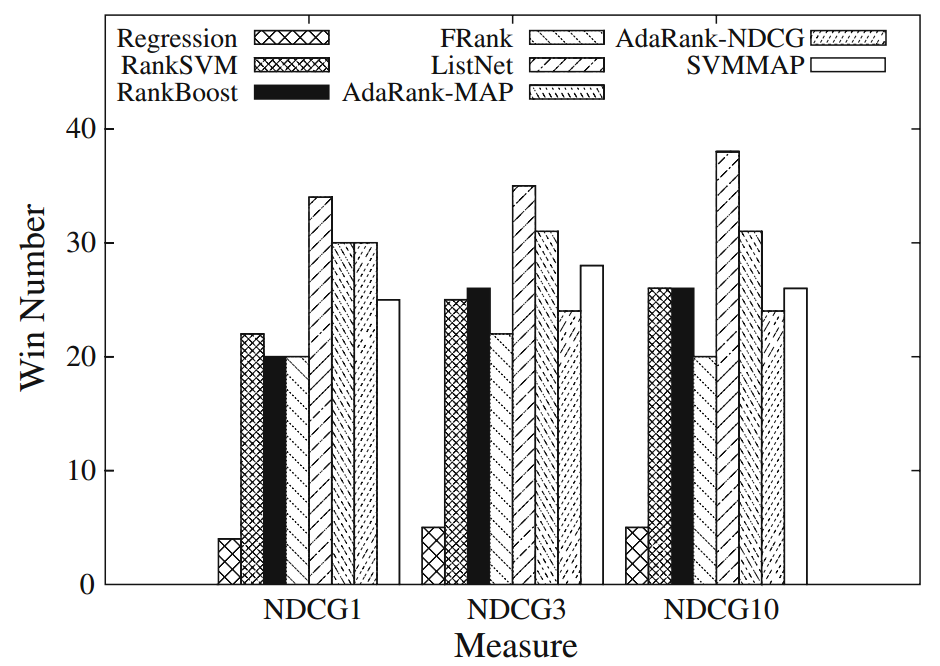
\includegraphics[scale=0.30]{gfx/ndcg_winning_number}
\caption{Comparison across the seven datasets in LETOR by \ac{nDCG}, obtained from Qin et al\cite{Qin2010}}
\label{fig:ndcg_winning_number}
\end{figure}

\begin{figure}[!h]
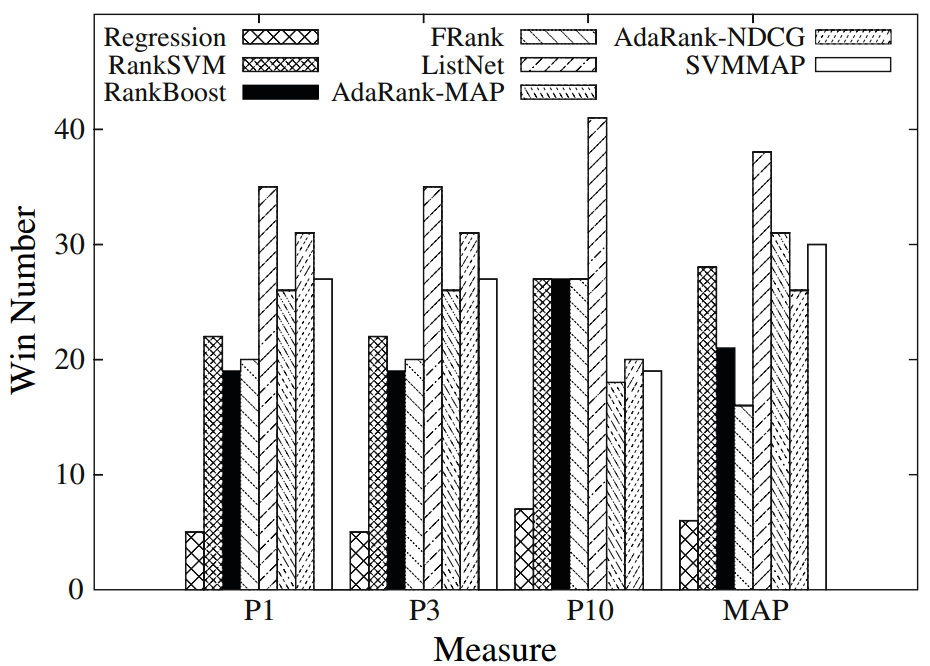
\includegraphics[scale=0.30]{gfx/map_winning_number}
\caption{Comparison across the seven datasets in LETOR by \ac{MAP}, obtained from Qin et al\cite{Qin2010}}
\label{fig:map_winning_number}
\end{figure}

I will describe the performance of the algorithms that were evaluated on LETOR3.0 after publication of the LETOR paper by Qin et al\cite{Qin2010} as listed on the LETOR website\footnote{http://research.microsoft.com/en-us/um/beijing/projects/letor/letor3baseline.aspx} by comparing their performance with the ListNet baseline. We will consider those methods to be better than ListNet when they beat the ListNet baseline in at least four of the seven datasets in \ac{nDCG} value. Note that this does not necessarily imply that these methods would have scored a higher \ac{nDCG} winning number than ListNet. Table \ref{tbl:LETOR_ListNet} shows the ListNet performance on the seven LETOR datasets in terms of \ac{nDCG}@10 and \ac{MAP}.
\begin{table}
\begin{tabular}{l|ll}
 & \ac{nDCG}@10 & \ac{MAP} \\ 
 \hline
TD2003 & 0.348 & 0.2753 \\ 
TD2004 & 0.317 & 0.2231 \\ 
NP2003 & 0.801 & 0.6895 \\ 
NP2004 & 0.812 & 0.6720 \\ 
HP2003 & 0.837 & 0.7659 \\ 
HP2004 & 0.784 & 0.6899 \\ 
OHSUMED & 0.441 & 0.4457 \\ 
\end{tabular}
\caption{Performance of ListNet on LETOR}
\label{tbl:LETOR_ListNet}
\end{table}

\begin{table}
\begin{tabular}{l|p{1.2cm}p{1.2cm}p{1.2cm}p{1.4cm}||l}
 & \rotatebox{55}{Regression + L2 regulatisation} & \rotatebox{55}{RankSVM-Primal} &\rotatebox{55}{RankSVM-Struct} & \rotatebox{55}{SmoothRank} & \rotatebox{55}{ListNet} \\
 \hline
TD2003 & 0.3297 & 0.3571 & 0.3467 & 0.3367 & 0.348 \\ 
TD2004 & 0.2832 & 0.2913 & 0.3090 & 0.3343 & 0.317 \\ 
NP2003 & 0.8025 & 0.7894 & 0.7955 & 0.7986 & 0.801 \\ 
NP2004 & 0.8040 & 0.7950 & 0.7977 & 0.8075 & 0.812 \\ 
HP2003 & 0.8216 & 0.8180 & 0.8162 & 0.8325 & 0.837 \\ 
HP2004 & 0.7188 & 0.7720 & 0.7666 & 0.8221 & 0.784 \\ 
OHSUMED & 0.4436 & 0.4504 & 0.4523 & 0.4568 & 0.441 \\ 
\# winning datasets & 2 & 2 & 1 & 3 & - \\ 
\end{tabular}
\caption{Comparison of algorithms recently evaluated on LETOR3.0 with the ListNet baselines}
\label{tbl:LETOR_recently_added}
\end{table}
\section{LETOR4.0}
\subsection{Results}

\chapter{MSLR-WEB10k/MSLR-WEB30k}
Contrary to the Yahoo! Learning to Rank Challenge dataset, the MSLR-WEB30k provides detailed feature descriptions. The MSLR-WEB30k dataset however contains no proprietary features but only features that are commonly used in the research community.
\section{Results}

\chapter{Selecting Learning-to-Rank methods}
The Accuracies of the Learning-to-Rank methods described in the preceding chapters must only be compared within the benchmark and not between benchmarks for the following reasons:
\begin{enumerate}
\item Differences in feature sets between data sets detract from fair comparison
\item Although the \ac{nDCG} definition is unambiguous, Busa-Fekete et al\cite{Busa-Fekete2012} found that \ac{nDCG} evaluation tools of benchmark data sets produced different scores
\end{enumerate}